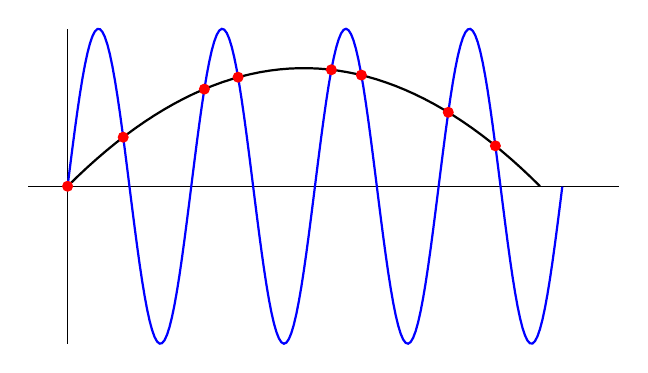
\begin{tikzpicture}

\draw (-0.5, 0) -- (7, 0);
\draw (0, -2) -- (0, 2);

\draw [samples=200, domain=0:2*pi, blue, thick] plot ( \x, {2 * sin(4*\x r)} );

\draw [samples=50, domain=0:6, thick] plot ( \x, { - \x * (\x - 6) / 6 } );

% points calculated with sage: find_root(2*sin(4*x)==-x * (x-6)/6, 2.5, 3.7 )
% and manually tweaking the limits so that the bisection algorithm finds each zero
\foreach \x in { 0, 0.7062 , 1.737, 2.165, 3.731, 3.3498, 4.8346 , 5.4329 }
{
	\fill[red] (\x, {2* sin(4*\x r) }) circle(2pt);
}

\end{tikzpicture}